% !Tex Program = xelatex
% -*-coding: utf-8 -*-
\documentclass[12pt,onecolumn]{report}

% 中文
\usepackage[BoldFont,SlantFont]{xeCJK}
\xeCJKsetemboldenfactor{1}%只对随后定义的CJK字体有效
\setCJKfamilyfont{hei}{SimHei}
\xeCJKsetemboldenfactor{4}
\setCJKfamilyfont{song}{SimSun}
\xeCJKsetemboldenfactor{4}
\setCJKfamilyfont{fs}{FangSong}
\setCJKfamilyfont{kai}{KaiTi}
\setCJKfamilyfont{li}{LiSu}
\setCJKfamilyfont{xw}{STXinwei}
\setCJKmainfont[BoldFont=SimHei]{SimSun}
\setCJKmonofont{SimSun}
\setCJKsansfont{SimSun}

\newcommand{\hei}{\CJKfamily{hei}}      % 黑体
\newcommand{\song}{\CJKfamily{song}}    % 宋体   (Windows 自带simsun.ttf)
\newcommand{\fs}{\CJKfamily{fs}}        % 仿宋体 (Windows 自带simfs.ttf)
\newcommand{\kai}{\CJKfamily{kai}}      % 楷体   (Windows 自带simkai.ttf)
\newcommand{\li}{\CJKfamily{li}}        % 隶书   (Windows自带simli.ttf)
\newcommand{\xw}{\CJKfamily{xw}}        % 隶书   (Windows自带simli.ttf)

% \AmSTeX\ 宏包,用来排出更加漂亮的公式。
\usepackage{amsmath}
% 定理类环境宏包,其中 \pkg{amsmath} 选项用来兼容 \AmSTeX\ 的宏包
\usepackage[amsmath,thmmarks,hyperref]{ntheorem}
\usepackage{amssymb}
% 添加字体
\usepackage[defaultsups]{newtxtext}
\usepackage{newtxmath}
\usepackage{courier}
% 图形支持宏包
\usepackage{graphicx}
% 插入pdf
\usepackage{pdfpages}
\includepdfset{fitpaper=true}
% 更好的列表环境。
\usepackage{enumitem}       %使用enumitem宏包,改变列表项的格式
\usepackage{environ}
% 禁止 \LaTeX 自动调整多余的页面底部空白,并保持脚注仍然在底部。
% 脚注按页编号。
\usepackage[bottom,perpage,hang]{footmisc}
\raggedbottom
% 脚注格式。
\usepackage{pifont}
% 表格控制
\usepackage{longtable}
\usepackage{booktabs}
% 参考文献引用宏包
\usepackage[sort&compress]{natbib}
% 生成有书签的 pdf 及其开关,请结合 gbk2uni 避免书签乱码。
\usepackage{hyperref}
\hypersetup{
  CJKbookmarks=true,
  linktoc=all,
  bookmarksnumbered=true,
  bookmarksopen=true,
  bookmarksopenlevel=1,
  breaklinks=true,
  colorlinks=false,
  plainpages=false,
  pdfborder=0 0 0}
% 设置 url 样式,与上下文一致
\urlstyle{same}
% 版芯设置
\usepackage{geometry}
\geometry{
  centering,
  text={150true mm,236true mm},
  left=30true mm,
  head=5true mm,
  headsep=2true mm,
  footskip=0true mm,
  foot=5.2true mm
}
% 利用 \pkg{fancyhdr} 设置页眉页脚。
\usepackage{fancyhdr}
% 其他包,表格、数学符号包
\usepackage{tabularx}
\usepackage{varwidth}
% 此处changepage环境用来控制索引页面的左右边距,规范中给出的示例的边距要大于正文。
\usepackage{changepage}
% 多栏结构在文中用begin{multicols}{2}end{multicols}
\usepackage{multicol,multienum}
% 允许上一个section的浮动图形出现在下一个section的开始部分,还提供\FloatBarrier命
% 令,使所有未处理的浮动图形立即被处理
\usepackage[below]{placeins}
% 支持子图 %centerlast 设置最后一行是否居中
\usepackage{subfigure}
% 支持双语标题
\usepackage[subfigure]{ccaption}
% 根据我工规定,正文小四号 (12bp) 字,行距为固定值3--4mm。
\renewcommand\normalsize{%
  % \@setfontsize\normalsize{12bp}{\ifhit@glue 20.50398bp \@plus 2.83465bp \@minus 0bp\else 20.50398bp\fi}%
  \abovedisplayskip=8pt
  \abovedisplayshortskip=8pt
  \belowdisplayskip=\abovedisplayskip
  \belowdisplayshortskip=\abovedisplayshortskip}
% 根据习惯定义字号。用法:\cs{hit@def@fontsize}\marg{字号名称}\marg{磅数}避免了
% 字号选择和行距的紧耦合。所有字号定义时为单倍行距,并提供选项指定行距倍数。
\def\hit@def@fontsize#1#2{%
  \expandafter\newcommand\csname #1\endcsname[1][1.3]{%
    \fontsize{#2}{##1\dimexpr #2}\selectfont}}
\hit@def@fontsize{dachu}{58bp}
\hit@def@fontsize{chuhao}{42bp}
\hit@def@fontsize{xiaochu}{36bp}
\hit@def@fontsize{yihao}{26bp}
\hit@def@fontsize{xiaoyi}{24bp}
\hit@def@fontsize{erhao}{22bp}
\hit@def@fontsize{xiaoer}{18bp}
\hit@def@fontsize{sanhao}{16bp}
\hit@def@fontsize{xiaosan}{15bp}
\hit@def@fontsize{sihao}{14bp}
\hit@def@fontsize{banxiaosi}{13bp}
\hit@def@fontsize{xiaosi}{12bp}
\hit@def@fontsize{dawu}{11bp}
\hit@def@fontsize{wuhao}{10.5bp}
\hit@def@fontsize{xiaowu}{9bp}
\hit@def@fontsize{liuhao}{7.5bp}
\hit@def@fontsize{xiaoliu}{6.5bp}
\hit@def@fontsize{qihao}{5.5bp}
\hit@def@fontsize{bahao}{5bp}
% 利用 \pkg{enumitem} 命令调整默认列表环境间的距离,以符合中文习惯。
\setlist{nosep}
% 允许太长的公式断行、分页等。
\allowdisplaybreaks[4]
\predisplaypenalty=0  %公式之前可以换页,公式出现在页面顶部
\postdisplaypenalty=0
% 公式编号设置
\renewcommand{\theequation}{\arabic{section}.\arabic{equation}}
% 定理标题使用黑体,正文使用宋体,冒号隔开。
\theorembodyfont{\normalfont}
\theoremheaderfont{\normalfont\hei}
\theoremsymbol{\ensuremath{\square}}
\newtheorem*{proof}{证明}
\theoremstyle{plain}
\theoremsymbol{}
\theoremseparator{}
\newtheorem{assumption}{假设}[section]
\newtheorem{definition}{定义}[section]
\newtheorem{proposition}{命题}[section]
\newtheorem{lemma}{引理}[section]
\newtheorem{theorem}{定理}[section]
\newtheorem{axiom}{公理}[section]
\newtheorem{corollary}{推论}[section]
\newtheorem{exercise}{练习}[section]
\newtheorem{example}{例}[section]
\newtheorem{remark}{注释}[section]
\newtheorem{problem}{问题}[section]
\newtheorem{conjecture}{猜想}[section]
% 各种单位
\usepackage{siunitx}
\sisetup{group-minimum-digits=4, group-separator= \hspace{0.25em}}
\sisetup{detect-weight,detect-mode,detect-family}
% 处理数学公式中的黑斜体的宏包
\usepackage{bm}
% 不同于 \mathcal \mathfrak 之类的英文花体字体
\usepackage{mathrsfs}
% 支持彩色
\usepackage{xcolor}
\definecolor{colorzero}{rgb}{0, 0, 0}
\definecolor{colorone}{rgb}{1, 0, 0}
\definecolor{colortwo}{rgb}{0, 0, 1}
\definecolor{colorthree}{rgb}{0, 1, 0}
% 图形和表格的控制旋转
\usepackage{rotating}
% 算法的宏包,注意宏包兼容性,先后顺序为float、hyperref、algorithm(2e),否则无法
% 生成算法列表。
\usepackage[algoruled,linesnumbered]{algorithm2e}
% 排版源码所使用的环境。
\usepackage{listings}
\lstset{
  language    = python,
  breaklines  = true,
  captionpos  = b,
  tabsize     = 4,
  numbers     = left,
  columns     = fullflexible,
  keepspaces  = true,
  frame       = shadowbox,
  commentstyle = \color[RGB]{0,128,0},
  keywordstyle = \color[RGB]{0,0,255}\bfseries,
  basicstyle   = \scriptsize\ttfamily,
  rulesepcolor = \color{red!20!green!20!blue!20},
  showstringspaces = false,
  breakatwhitespace = false,
}

% 作图
\usepackage{tikz}
\usetikzlibrary{graphs, positioning, quotes, shapes.geometric}

% 首行缩进
\usepackage{indentfirst}
\setlength{\parindent}{2em}

\usepackage{float}
\usepackage{diagbox}
\usepackage{setspace}
\usepackage{zhnumber}
\usepackage{titlesec}

\renewcommand\thechapter{\zhnum{chapter}}
\renewcommand\thesection{\arabic{section}}

\titleformat{\chapter}{\centering\Huge\bfseries}{第\,\thechapter\,章}{1em}{}
% \titleformat{\section}{\raggedright\Large\bfseries}{\thesection\,}{1em}{}
% \titleformat{\subsection}{\raggedright\large\bfseries}{\,\thesubsection\,}{1em}{}
% \titleformat{\subsubsection}{\raggedright\large\bfseries}{\,\thesubsubsection\,}{1em}{}

\graphicspath{{figures/}}

\pagestyle{fancy}
\fancyhead[L]{\song\xiaowu[0]{cycleke}}
\fancyhead[C]{\song\xiaowu[0]{哈尔滨工业大学}}
\fancyhead[R]{\song\xiaowu[0]{人工智能导论实验报告}}
\fancyfoot[C]{\xiaowu-~\thepage~-}

\renewcommand{\today}{\number\year{年}\number\month{月}\number\day{日}}
\renewcommand{\contentsname}{\centering 目录}
\renewcommand{\figurename}{图}
\renewcommand{\tablename}{表}
\numberwithin{figure}{section}

\renewcommand{\baselinestretch}{1.25}
\renewcommand{\abstractname}{\hei{\huge {摘\quad 要}}} %更改摘要二字的样式
\newcommand{\M}[1]{\mathbf{#1}}
\setcounter{secnumdepth}{4}

\begin{document}

\begin{titlepage}
  \centering

  \kai\xiaochu{}
  \makebox[350bp][s]{人工智能导论实验报告}

  \vspace{5\baselineskip}

  \hei\xiaosan{}
  \makebox[60bp][s]{题目}~\underline{\makebox[150bp][s]{人工智能实验}} \\
  \makebox[60bp][s]{姓名}~\underline{\makebox[150bp][s]{c y c l e k e}} \\
  \makebox[60bp][s]{学号}~\underline{\makebox[150bp][s]{x x x x x x x}} \\
  \makebox[60bp][s]{院系}~\underline{\makebox[150bp][s]{计算学部}} \\
  \makebox[60bp][s]{专业}~\underline{\makebox[150bp][s]{数据科学与大数据技术}} \\
  \makebox[60bp][s]{指导老师}~\underline{\makebox[150bp][s]{x x x}} \\
  \makebox[60bp][s]{同组成员}~\underline{\makebox[150bp][s]{x x x, x x x, x x x}} \\

  \vspace{3\baselineskip}
  \begin{figure}[ht]
    \centering
    
\includegraphics[width=0.6\linewidth,centering]{figures/school.eps}
  \end{figure}
\end{titlepage}


\clearpage
\tableofcontents
\clearpage

\setcounter{chapter}{-1}
\chapter{前言}
\section{实验环境说明}
在本次实验中,我们小组使用的环境如下:
\begin{itemize}[fullwidth,itemindent=\parindent]
\item 操作系统: Arch Linux x86\_64
\item 内存:4GB @ 2666MHz $\times$ 2
\item CPU: Intel i5-8250U (8) @ 3.400GHz
\item Golang 编译器版本: go version go1.15.4 linux/amd64
\item Python 解释器版本: Python 2.7.18
\item C++ 编译器版本: gcc (GCC) 10.2.0
\end{itemize}

\chapter{实验一~知识表示}
\section{问题描述}
\subsection{基本要求}
实验一要求我们参照课程第二部分讲授的知识表示的方式,
运用包括产生式系统、框架系统、语义网络等方法求解猴子取香蕉的问题。

\subsection{猴子取香蕉问题}
一个房间里,天花板上挂有一串香蕉,
有一只猴子可在房间里任意活动(到处走动,推移箱子,攀登箱子等)。
设房间里还有一只可被猴子移动的箱子,
且猴子登上箱子时才能摘到香蕉,
问猴子在某一状态下(设猴子位置为A,香蕉位置在B,箱子位置为C),如何行动可摘取到香蕉。

\section{算法介绍}

\subsection{产生式表示法}
产生式表示法是一种知识表示方法,
其基本形式为$P \to Q$(或 IF P THEN Q)。
其中, P 是产生式的前提,也称为前件,它给出了该产生式可否使用的先决条件。
Q 是一组结论或操作,也称为后件,它指出当P满足时,应该推出的结论或应该执行的动作。

产生式系统的基本结构包括如下三个部分:
\begin{itemize}[fullwidth,itemindent=\parindent]
\item 综合数据库,
  用于存放推理过程的各种当前信息
  以及作为推理过程选择可用规则的依据。
\item 规则库,
  用于存放推理所需要的所有规则,
  是整个产生式系统的知识集,
  是产生式系统能够进行推理的根本。
\item 控制系统,
  用于控制整个产生式系统的运行,
  决定问题求解过程的推理线路。
\end{itemize}

\subsection{解决方案}
根据产生式表示法,我们定义如下部分
\begin{itemize}[fullwidth,itemindent=\parindent]
\item 综合数据库: (Monkey, Banana, Box, On, Have),其中
  Monkey 表示猴子的位置,
  Banana 表示香蕉的位置,
  Box 表示箱子的位置,
  On 表示猴子是否在箱子上(0 表示否,1 表示是),
  Have 表示猴子有没有抓到香蕉(同上)。
\item 规则数据库包含的规则如下:
  \begin{enumerate}[fullwidth,itemindent=\parindent,label=r\arabic*:]
  \item IF (x, y, z, 0, 0) THEN (w, y, z, 0, 0)
  \item IF (x, y, x, 0, 0) THEN (z, y, z, 0, 0)
  \item IF (x, y, x, 0, 0) THEN (x, y, x, 1, 0)
  \item IF (x, y, x, 1, 0) THEN (x, y, x, 0, 0)
  \item IF (x, x, x, 1, 0) THEN (x, x, x, 1, 1)
  \end{enumerate}
\end{itemize}

根据问题,确定终止状态是猴子摘到香蕉,
所以终止状态为 (C, C, C, 1, 1),
而初始状态为 (A, B, C, 0, 0)。
控制系统需要做的就是
根据初始状态和规则库中的规则,
不断地产生新的状态,直到到达目标状态为止。

\section{算法实现}
在本实验中,
我们使用 Golang (版本 1.15.4 linux/amd64) 编写程序,
程序编译运行的结果如下:
\begin{figure}[htbp]
  \centering
  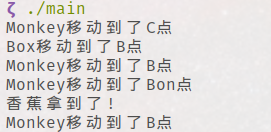
\includegraphics{figures/monkey.png}
  \caption{实验一运行结果}
\end{figure}

\section{讨论及结论}
该实验让我们了解了如何利用知识表示方法解决一个具体的问题,
知道了知识表示方法解决问题的具体步骤。

在综合了各个表示方法的优缺点后,我们最终选择了产生式的表示方法。
通过构建了产生式的组成(综合数据库、规则库以及控制系统),
并定义了初始状态和目标状态,
我们最终找到了一条从初始状态到目标状态的路径进而
解决了猴子取香蕉问题。

\chapter{实验二~搜索策略}
\section{问题描述}
实验二要求采用且不限于课程第四章内各种搜索算法,
编写一系列吃豆人程序解决下面列出的 8 个问题,
包括到达指定位置以及有效地吃豆等。
具体的八个问题如下:
\begin{enumerate}[fullwidth,itemindent=\parindent,label=问题\arabic*:]
\item 应用深度优先算法找到一个特定的位置的豆
\item 应用宽度优先算法找到一个特定的位置的豆
\item 应用代价一致算法找到一个特定的位置的豆
\item 应用A* 算法找到一个特定的位置的豆
\item 找到所有的角落
\item 角落问题(启发式)
\item 吃掉所有的豆子
\item 次最优搜索
\end{enumerate}

在本实验中,
我们要使用深度优先算法(DFS),宽度优先算法(BFS),
代价一致算法(UCS),A* 算法等搜索算法来为吃豆人规划路径以完成特定的目标。
其中前四个问题为本质是实现一个朴素的搜索算法,
后四个问题则是为具体的搜索问题设计不同的搜索策略和估价函数。

\section{算法介绍}
在本章,我们将针对简单介绍实验二吃豆人中的八个问题,
分析各个问题并说明解决问题的方法及算法实现。

\subsection{问题一~应用深度优先算法找到一个特定的位置的豆}
\subsubsection{问题描述}
在本问题以及后续的三个问题中,
我们需要为吃豆人规划一条在给定迷宫中从特定起点到特定终点的路径。
在问题一中,我们需要使用深度优先搜索算法求解该问题。

值得注意的是,前四个问题的问题其实是相似的,
唯一的不同就是其使用的搜索算法不同。
因为不同的搜索方法的不同之处仅仅在于 open 表的排序不同,
因此我们可以使用一个通用的搜索算法解决问题一到四,
通过修改数据结构来实现不同的搜索算法。

\subsubsection{算法实现}
我们首先需要实现一个通用的搜索算法,
实验大纲中附录的伪代码如下:
\begin{figure}[h]
  \centering
  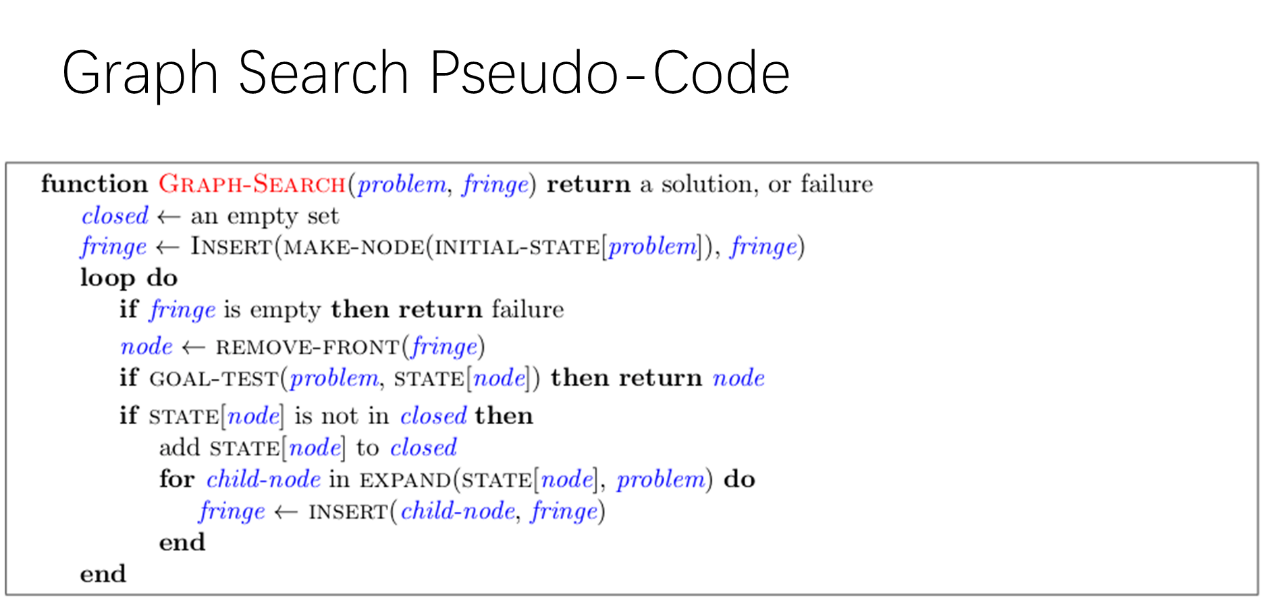
\includegraphics{figures/general_search.png}
  \caption{通用搜索算伪代码}
\end{figure}

在具体实现的过程中,
我们使用一个三元组来代表一个 node,
分别存储当前状态的位置,路径(即从初始状态到达本状态所要执行的操作序列)和到达当前点的代价。
由于 PriorityQueue 的 push 方法同其他数据结构不同,所以对其需要特判。
为了实现后面的 A* 算法,我们需要传入一个 heuristic 参数来进行估价,
其默认值为 nullHeuristic,该函数始终返回 0(即不进行估计)。
如果不存在一条从起点到终点的路径,那么代码会返回特殊值 None 表示无解。
具体的代码实现如下:
\begin{lstlisting}[language=python]
def generic_search(problem, open_table_type, heuristic=nullHeuristic):
    """
      problem: the problem to solve
      open_table_type: the type of the open table to imply different search algorithm
      heuristic: the heuristic function

    A general search method.
    """
    open_table = open_table_type()
    is_priority_queue = isinstance(open_table, util.PriorityQueue)

    def push_to_open_table(state, actions, cost):
        if is_priority_queue:
            open_table.push((state, actions, cost),
                            cost + heuristic(state, problem))
        else:
            open_table.push((state, actions, cost))

    closed_table = set()
    push_to_open_table(problem.getStartState(), [], 0)
    while not open_table.isEmpty():
        state, actions, cost = open_table.pop()
        if state in closed_table: continue
        closed_table.add(state)
        if problem.isGoalState(state):
            return actions
        for successor, action, step_cost in problem.getSuccessors(state):
            push_to_open_table(successor, actions + [action], cost + step_cost)
    return None
\end{lstlisting}

在深度优先搜索算法中,
程序会首先扩展最新产生的(即最深的)节点,
当前结点无法拓展时才会回溯到祖先结点,采用的是后生成的节点先扩展的策略。
所以深度优先搜索算法的 open 表应该使用先进后出(FILO)的栈结构来实现。
基于前面已经实现的通用的搜索算法,我们只需要将 open\_table\_type 设置为栈即可。

\begin{lstlisting}[language=python]
def depthFirstSearch(problem):
    ....
    return generic_search(problem, util.Stack)
\end{lstlisting}

\subsection{问题二~应用宽度优先算法找到一个特定的位置的豆}
\subsubsection{问题描述}
在本问题中,
我们需要使用深度优先搜索算法
为吃豆人规划一条在给定迷宫中从特定起点到特定终点的路径。

\subsubsection{算法实现}
宽度优先搜索算法的基本思想是
从初始结点开始扩展,当且仅当第 n 层的结点全部扩展完之后,才会开始扩展下一层结点,
采用的时先生成的结点先扩展的策略。
所以宽度优先搜索算法的 open 表应该使用先进先出(FIFO)的队列结构来实现。
基于前面已经实现的通用的搜索算法,我们只需要将 open\_table\_type 设置为队列即可。

\begin{lstlisting}[language=python]
def breadthFirstSearch(problem):
    ....
    return generic_search(problem, util.Queue)
\end{lstlisting}

\subsection{问题三~应用代价一致算法找到一个特定的位置的豆}
\subsubsection{问题描述}
前面的各种搜索策略中,
实际都假设状态空间中各边的代价都相同,且都为一个单位量,从而可以用路径长度来代替路径的代价。
但实际问题中,这种假设不现实,它们的状态空间中的各个边的代价不可能完全相同。
为此,我们需要在搜索树中给每条边标上其代价。
这种边上有代价的树称为代价树。

在本问题中,我们就需要使用代价一致搜索算法
为吃豆人规划一条在给定路径带权的迷宫中从特定起点到特定终点的最短路径。

\subsubsection{算法实现}
代价一致搜索算法是在宽度优先搜索上进行扩展的,
它的基本原理是:代价一致搜索总是扩展代价最小的节点。
一个点的代价等于前一节点的代价加上从前一结点到当前节点的代价。

相比于宽度优先搜索算法,
代价一致搜索不是沿着等长度路径逐层进行扩展,而是沿着等代价路径逐层进行扩展。
该算法的 open 表需要维护一个有序集合,支持每次取出最小值元素的操作。
所以我们使用优先队列来实现这种 open 表。
基于前面已经实现的通用的搜索算法,我们只需要将 open\_table\_type 设置为优先队列即可。

\begin{lstlisting}[language=python]
def uniformCostSearch(problem):
    ....
    return generic_search(problem, util.PriorityQueue)
\end{lstlisting}

\subsection{问题四~应用 A* 算法找到一个特定的位置的豆}
\subsubsection{问题描述}
在本问题中,我们就需要使用 A* 算法
为吃豆人规划一条在给定路径带权的迷宫中从特定起点到特定终点的最短路径。

\subsubsection{算法实现}
A* 算法是一种启发式搜索的方法,
该算法综合了宽度优先算法和迪杰斯特拉算法算法的优点:
在进行启发式搜索提高算法效率的同时,可以保证找到一条最优路径(基于评估函数)。

在此算法中,如果以$g(n)$表示从起点到任意顶点$n$的实际距离,
$h(n)$表示顶点$n$到目标顶点的估算距离(根据所采用的评估函数的不同而变化)
,那么 A* 算法的估算函数为$f(n) = g(n) + h(n)$。

在 A* 算法中,我们需要优先扩展估算函数最小的节点,
所以选择优先队列作为 open 表的数据结构。

\begin{lstlisting}[language=python]
def aStarSearch(problem, heuristic=nullHeuristic):
    ....
    return generic_search(problem, util.PriorityQueue)
\end{lstlisting}

\subsection{问题五~找到所有的角落}
\subsubsection{问题描述}
在本问题中,我们需要实现 CornersProblem 类,
用来表示“让吃豆人将以最短的路径找到迷宫的四个角落”这一问题。
我们需要为这个类设计出对应的状态并写出对应的目标状态判定和后即状态获取。

\subsubsection{算法实现}
对于本问题,显然我们不能直接使用位置来表示当前状态。
我们需要使用额外的变量来存储四个角落的访问状态。
为此,我将每个状态设计为一个包含位置和角落的访问状态的二元组。
四个角落的访问状态使用一个整数的四个比特位表示,
使用 1 表示对应位置访问过, 0 表示对应位置没有访问过。
该整数的初始值为 0,而目标状态就是所有该整数为 $2^{4} - 1 = 15$的状态。

\begin{lstlisting}[language=python]
def isGoalState(self, state):
    ....
    return state[1] == self.ALL_GOT
\end{lstlisting}

此外,getSuccessors 方法也是本部分的一个核心。
由于在状态表示中增加了对角落状态的表示,
所以在生成后继状态时也要考虑这部分是否会变化。
考虑生成的后继节点,若后继节点是未到达过的角落位置,
则在该后继的表示访问状态的整数中,要将对应的比特位置为 1,表示已经到达过该角落。

\begin{lstlisting}[language=python]
def getSuccessors(self, state):
    ....
    x, y = state[0]
    visited = state[1]
    successors = []
    for action in [
            Directions.NORTH, Directions.SOUTH, Directions.EAST,
            Directions.WEST
    ]:
        dx, dy = Actions.directionToVector(action)
        nextx, nexty = int(x + dx), int(y + dy)
        hitsWall = self.walls[nextx][nexty]
        if hitsWall: continue
        successor_position = (nextx, nexty)
        successor_visited = visited
        for i, position in enumerate(self.corners):
            if successor_position == position:
                successor_visited |= 1 << i
        successor = (successor_position, successor_visited)
        successors.append((successor, action, 1))

    self._expanded += 1  # DO NOT CHANGE
    return successors
\end{lstlisting}

\subsection{问题六~角落问题(启发式)}
\subsubsection{问题描述}
本问题要求我们构建合适的启发函数,
完善 cornersHeuristic 函数,实现使用启发式函数来解决问题五中的角落问题。

大纲要求使用 A* 启发式搜索算法来解决角落问题,
并且出设计一个非平凡且一致的启发式函数 cornersHeuristic,
以通过扩展尽量少的节点访问所有四个角落。
其中非平凡且一致算启发式函数就是要求我们对于所有的非目标状态$n$,
设$h(n)$为$n$到达目标状态的真实代价,
$h^*(n)$为启发式函数估计的代价,那么$0 < h^*(n) \le h(n)$,且$h^*(goal) = 0$。
这样可以保证我们可以得到正确的最短路径。

\subsubsection{算法实现}
我设计的启发性函数的启发策略为
依次遍历四个角落中尚未访问的所有角落的排列,
按照排列的顺序访问四个结点,用宽度优先搜索算法
(即假设每条边的代价为 1)来估计两个结点的距离。

显然,两个结点间的距离是小于等于它们在迷宫中的真实距离的,
故上述启发式函数
\[h^{*}(n) = \min_{\text{所有排列}}\sum\text{BFS 距离}
  \le \min_{\text{所有排列}}\sum\text{真实距离} = h(n)\]

而对于非目标结点, $h^{*}(n) > 0$ 是显然的,
所以该启发式函数是非平凡且一致的。
为了提高程序的效率,我们使用一个字典来存储已计算的距离。
对应的代码实现如下,:

\begin{lstlisting}[language=python]
def cornersHeuristic(state, problem):
    ....
    position, visited = state
    left_corners = []
    for i, corner in enumerate(corners):
        if visited >> i & 1: continue
        left_corners.append(corner)

    dist = problem.distance

    def get_dist(x, y):
        if (x, y) in dist: return dist[(x, y)]
        if (y, x) in dist: return dist[(y, x)]
        d = mazeDistance(x, y, problem.startingGameState)
        dist[(x, y)], dist[(y, x)] = d, d
        return d

    if not left_corners: return 0

    import itertools
    min_distance = 10**9
    for order in itertools.permutations(left_corners):
        cost, pre = 0, position
        for corner in order:
            cost += get_dist(pre, corner)
            pre = corner
        min_distance = min(min_distance, cost)
    return min_distance
\end{lstlisting}

\subsection{问题七~吃掉所有的豆子}
\subsubsection{问题描述}
在本问题中,
多个食物不仅仅局限在角落出现,它们可能出现在任何地方。
本问题需要一个十分良好的非平凡且一致的启发式函数,
用尽可能少的步数,同时尽量扩展少的节点以找到一条可以获得所有的食物路径。

\subsubsection{算法实现}
一个始终走向距离其最近食物的吃豆人行走的路径不一定是最短路径。
因而在问题七中对走遍所有食物的总路径寻找下界是一件比较困难的事。
因而,我们考虑在所有剩余食物中选择具有代表性的食物,
使用该食物位置与吃豆人当前位置之间的距离来代表吃豆人到达目标所需要的代价下界。

我设计的启发性函数的启发策略为
当剩余的食物结点较少时,我们使用类似问题六的策略,枚举排列即可;
当剩余的食物结点较多时,我们先访问最近的结点,之后距离最近结点最远的结点。
因为我们一定是先吃完当前点附近的食物,再去吃最远处的食物。
因为我们只考虑了两个结点间的距离,远小于实际食物点间的距离,
所以我们的启发式函数$h^{*}(n) \le h(n)$,是非平凡且一致的。

为了提高程序的效率,类似问题六,
我们同样使用一个字典来存储已计算的距离。
对应的代码实现如下:

\begin{lstlisting}[language=python]
def foodHeuristic(state, problem):
    ....
    position, foodGrid = state
    foods = foodGrid.asList()
    dist = problem.heuristicInfo

    if not foods: return 0

    def get_distance(x, y):
        if (x, y) in dist: return dist[(x, y)]
        if (y, x) in dist: return dist[(y, x)]
        d = mazeDistance(x, y, problem.startingGameState)
        dist[(x, y)], dist[(y, x)] = d, d
        return d

    if len(foods) == 1: return get_distance(foods[0], position)

    if len(foods) < 9:
        vector = tuple(foods) + (position, )
        if vector in dist: return dist[vector]
        import random, itertools
        random.shuffle(foods)
        min_cost = 10**9
        for order in itertools.permutations(foods):
            pre, cost = position, 0
            for food in order:
                cost += get_distance(pre, food)
                if cost >= min_cost:
                    break
                pre = food
            if min_cost > cost:
                min_cost = cost
        dist[vector] = min_cost
        return min_cost

    d, closest = min([(get_distance(food, position), food) for food in foods])
    return d + max([get_distance(food, closest) for food in foods])
\end{lstlisting}

\subsection{问题八~次最优搜索}
\subsubsection{问题描述}
本问题要求实现一个优先吃最近的食物的路径规划算法,
需要我们实现 AnyFoodSearchProblem 类中的 isGoalState 方法
以及 ClosestDotSearchAgent 类中的 findPathToClosestDot 方法。

\subsubsection{算法实现}
通过阅读 ClosestDotSearchAgent 类下代码,
我们发现该问题类的运行逻辑是
不断的使用 findPathToClosestDot 寻找一条距离当前结点
最近的食物的路径并将该路径加入到答案路径之中,直到所有的食物均被吃完。
因而在 AnyFoodSearchProblem 类中,
我们定义将能够吃掉一个食物为对应的目标状态,
以使 findPathToClosestDot 方法在会吃到距离最近的食物。

isGoalState 的代码如下:
\begin{lstlisting}[language=python]
def isGoalState(self, state):
    x, y = state
    return self.food[x][y]
\end{lstlisting}

而在 findPathToClosestDot 方法中,
我们要给出吃豆人到最近的食物的actions列表,
因此使用宽度优先搜索算法进行搜索出
一条到达最近食物的最短的路径。

findPathToClosestDot 方法的代码如下:
\begin{lstlisting}[language=python]
def findPathToClosestDot(self, gameState):
    ....
    startPosition = gameState.getPacmanPosition()
    food = gameState.getFood()
    walls = gameState.getWalls()
    problem = AnyFoodSearchProblem(gameState)

    min_distance, ans = 10**9, None
    for pos in food.asList():
        if util.manhattanDistance(startPosition, pos) >= min_distance:
            continue
        prob = PositionSearchProblem(gameState,
                                     start=startPosition,
                                     goal=pos,
                                     warn=False,
                                     visualize=False)
        path = search.bfs(prob)
        distance = len(path)
        if distance < min_distance:
            ans = path
            min_distance = distance
    return ans
\end{lstlisting}

\section{算法实现}
本节给出运行 autograder.py 后对于每个问题的评分结果。
\begin{figure}[H]
  \centering
  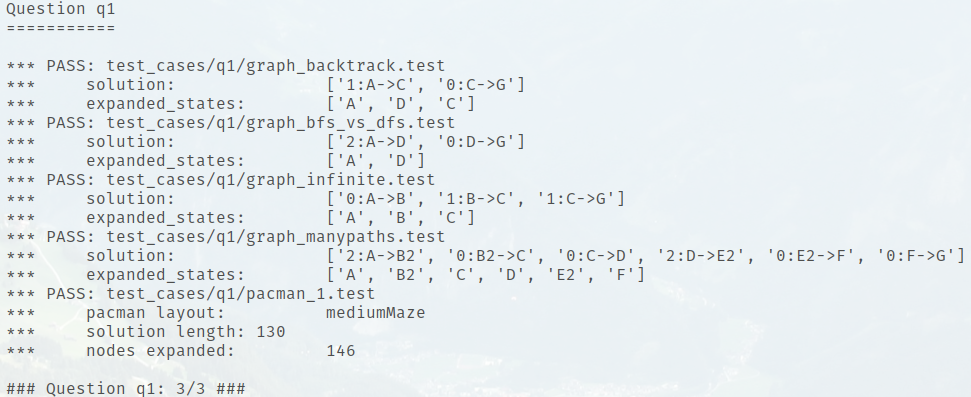
\includegraphics[width=\linewidth]{figures/q1.png}
  \caption{问题一运行结果}
\end{figure}

\begin{figure}[H]
  \centering
  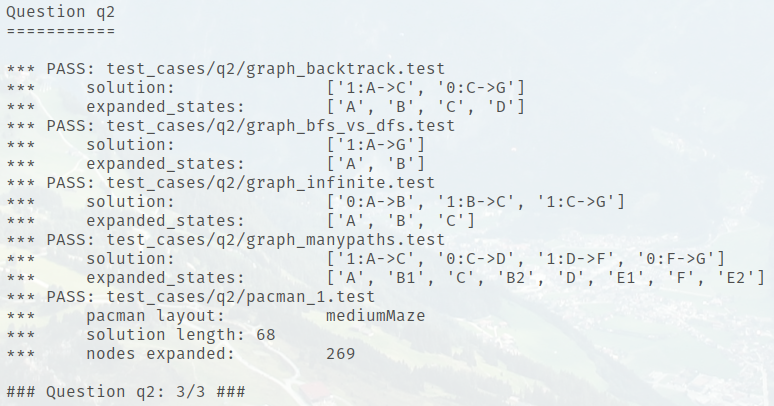
\includegraphics{figures/q2.png}
  \caption{问题二运行结果}
\end{figure}

\begin{figure}[H]
  \centering
  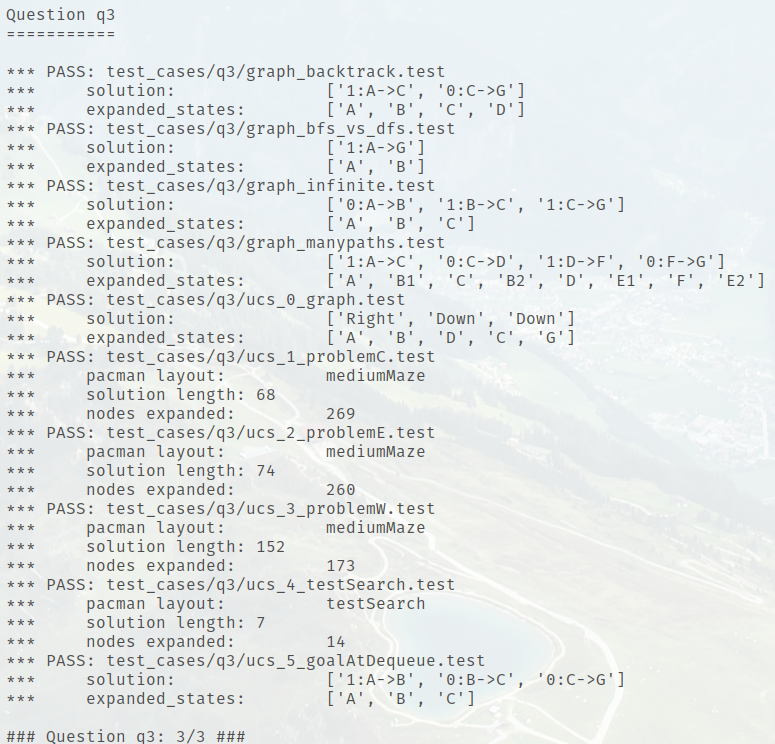
\includegraphics{figures/q3.png}
  \caption{问题三运行结果}
\end{figure}

\begin{figure}[H]
  \centering
  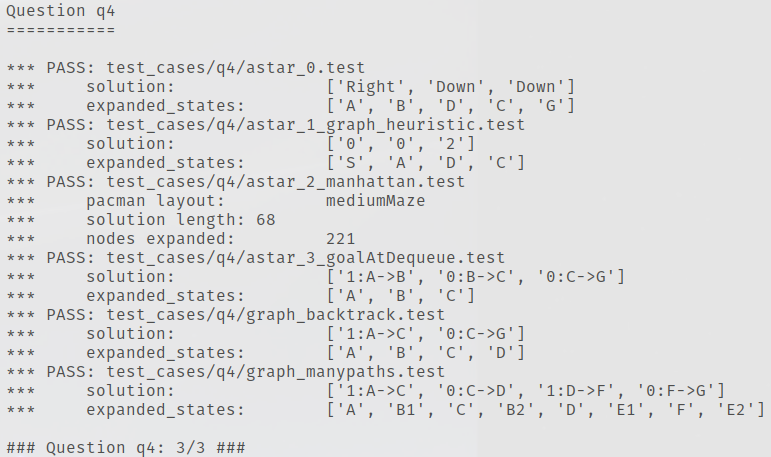
\includegraphics{figures/q4.png}
  \caption{问题四运行结果}
\end{figure}

\begin{figure}[H]
  \centering
  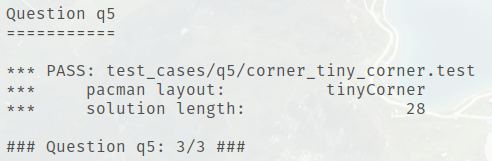
\includegraphics{figures/q5.png}
  \caption{问题五运行结果}
\end{figure}

\begin{figure}[H]
  \centering
  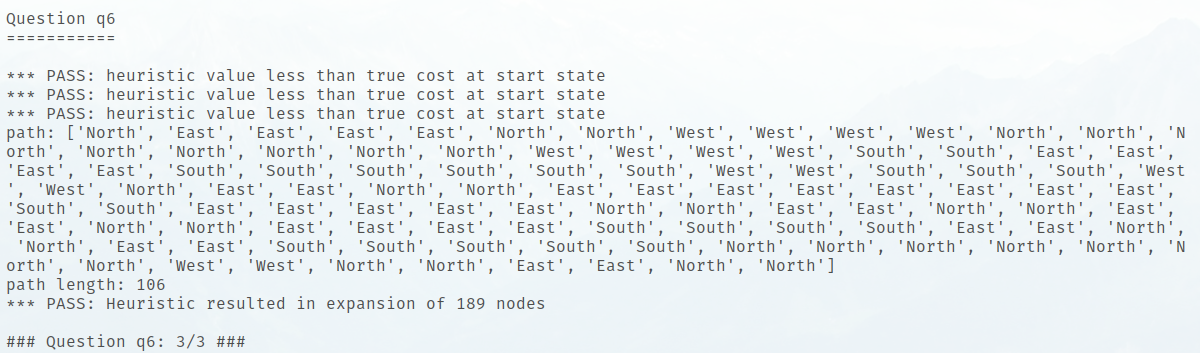
\includegraphics[width=\linewidth]{figures/q6.png}
  \caption{问题六运行结果}
\end{figure}

\begin{figure}[H]
  \centering
  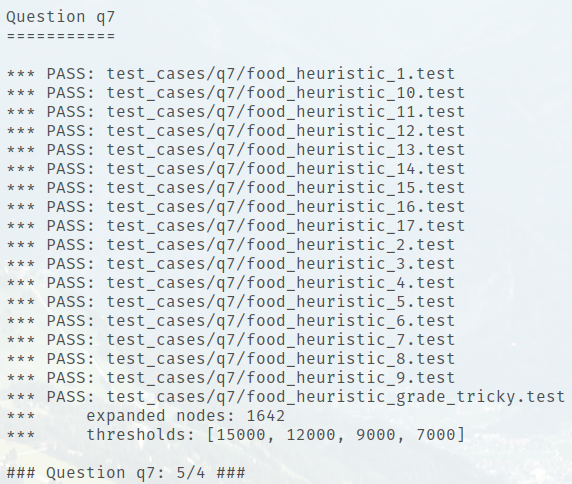
\includegraphics[width=0.4\linewidth]{figures/q7.png}
  \caption{问题七运行结果}
\end{figure}

\begin{figure}[H]
  \centering
  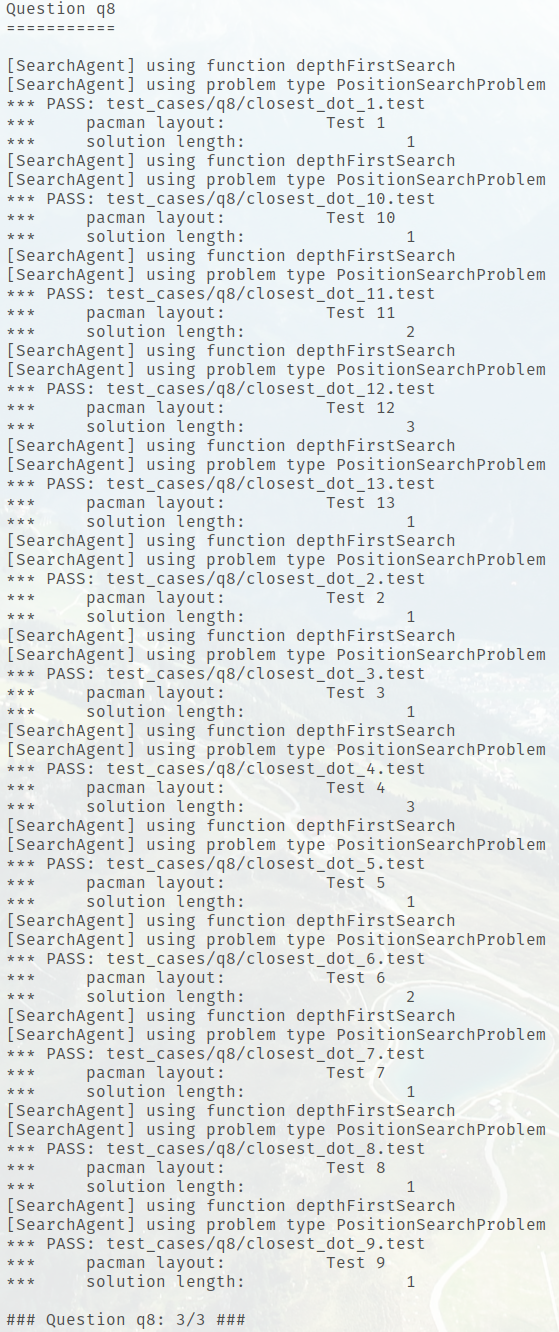
\includegraphics[width=0.4\linewidth]{figures/q8.png}
  \caption{问题八运行结果}
\end{figure}

\section{讨论及结论}
在本次实验中我们
实现了深度优先、宽度优先、代价一致、A* 这四种搜索算法,
同时也学习了启发式函数的选取要求和方法,通过优化启发式函数来提高搜索的效率。

本次实验可以说是一次很有意思的实验了。
本次前四个搜索算法,
由于仅仅是 open 表使用的数据结构不用,其他大部分都是一样的,
因此将四个算法写在了一起,组合成了一个函数,实现了抽象和复用。
后面四个问题是在前四个搜索算法已经写好的条件下计算的,
根据不同的要求,填写代码不同的部分并选择合适的搜索算法,
不断优先自己的启发式函数,最后实现一个满足条件的高效算法。
经过本次实验,我对搜索算法有了进一步的理解,掌握了一些优化启发式函数的方法。

\chapter{实验三~不确定性推理}
\section{问题描述}
\subsection{基本要求}
本实验要求我们参照课程第五部分讲授的贝叶斯网络完成。
实验会给定事件和事件之间的关系,并且给出每个事件的 CPT 图,
要求程序根据贝叶斯公式根据上述条件求出目标概率,编写程序实现基于贝叶斯网络的推理。
在这里用到的贝叶斯算法是建立在有向无环图和 CPT 表的技术上实现的。
\subsection{输入输出描述}
首先我们需要读入形如
\begin{lstlisting}
N

rv0	rv1	...	rvN-1
0	0	1	...	0
1	0	0	...	1
...
0	1	1	...	0

mat0

mat1

...

matN-1
\end{lstlisting}

在这里,
N	是贝叶斯网络中随机事件的数目,
rv 是随机事件的名字(字符串形式表示),
mat 是一个二维数组,分别表示从他的父亲到其本身的可能性概率。
第一个元素表示发生的概率,第二个元素表示不发生的概率,显然两个元素相加为 1。

在上述中 mat 即为 CPT 表(Conditional Probability Table),
其被设计为如下格式:
对于每个节点,如果他有 N 个父节点,
则其 CPT 表中有$2^N$列,我们记为标号$0 \ldots 2^{N}-1$。
其行序号的定义方法如下:
利用二进制分别表示对应的父亲为是否发生,
1为发生,0位不发生,
将得到的二进制数转化为十进制代表其对应的行号。

其次,编写程序对应的查询格式为:
$P(\text{rvQ} \vert \text{rvE1}=\text{val},\text{rvE2}=\text{val},\ldots)$,
rvQ 表示查询的条件的名字,
即在 $\text{rvE1}=\text{val},\text{rvE2}=\text{val}, \ldots$发生的条件下,rvQ发生的概率;
RvEx 表示条件的名称, 而后面的 val 为 true 或 false,分别表示发生和不发生。
最后,输出格式为两个数据分别表示
$P(\text{QueryVar}=\text{true} \vert \ldots)$	和 $P(\text{QueryVar}=\text{false} \vert \ldots)$。

\section{算法介绍}
\subsection{基本原理}
我们程序基本基于如下公式:
\begin{align}
  Z &= \sum_{q} P(Q, e_{1} \ldots, e_{k}) \\
  P(Q \vert e_{1} \ldots, e_{k}) &= \frac{1}{Z} P(Q, e_{1} \ldots, e_{k})
\end{align}

我们先求解出所有的$2^{N}$个事件的概率,得出联合概率表。
然后读入需求解的概率,
利用穷举法,计算相应的联合概率,
最后根据 CPT 图消去无关变量,归一化得到待求概率的解。

\subsection{代码实现}
我们在读入贝叶斯网络后,先根据贝叶斯网络和 CPT 图计算出每个事件的全概率,
将$N$个随机变量共$2^N$个事件编码为$N$位二进制数,
最高位为1代表第一个随机变量取值 (1 为真,0 为假),
次高位代表第二个随机变量的取值,以此类推。
对于每个事件,遍历每个随机变量,
提取出该随机变量的父节点的取值,查询 CPT 进行累乘,得到该事件的联合概率。
代码实现如下:

\begin{lstlisting}[language=c++]
void calculateTotalProbability() {
  int bound = 1 << n;
  total_probability.resize(bound, 1);
  for (int s = 0; s < bound; ++s) {
    double &poss = total_probability[s];
    for (int i = 0; i < n; ++i) {
      int index = 0;
      static auto get_bit = [&](int x) { return s >> (n - 1 - x) & 1; };

      for (int x : cpts[i].parents) index = index << 1 | get_bit(x);
      poss *= cpts[i].probabilities[index][get_bit(i)];
    }
  }
}
\end{lstlisting}

然后根据输入的待求解的概率,
提取出欲求解的随机变量与已知的随机变量取值,
将无关的变量消去,最后归一化即得到最终解。

\begin{lstlisting}[language=c++]
std::vector<double> calculateProbability(const std::vector<int> &vars) const {
  // var : 0: 假, 1: 真, 2: 求解, 3: 待消去
  assert(static_cast<int>(vars.size()) == n);

  int to_solve = 0, to_eliminate = 0;
  for (int x : vars) {
    to_solve += x == 2;
    to_eliminate += x == 3;
  }
  assert(to_solve == 1);

  int solve_case = 1 << to_solve;
  int eliminate_case = 1 << to_eliminate;

  std::vector<double> probability(solve_case, 0);
  for (int solve = 0; solve < solve_case; ++solve)
    for (int eliminate = 0; eliminate < eliminate_case; ++eliminate) {
      auto values = vars;
      int c_solve = to_solve, c_eliminate = to_eliminate, index = 0;
      for (int &x : values) {
        if (x == 2) x = solve >> (--c_solve) & 1;
        if (x == 3) x = eliminate >> (--c_eliminate) & 1;
        index = index << 1 | x;
      }
      probability[solve] += total_probability[index];
    }

  double sum = 0;
  for (auto &x : probability) sum += x;
  for (auto &x : probability) x /= sum;
  return probability;
}
\end{lstlisting}

\section{算法实现}
我们使用如下代码测试我们实现的 bayesian\_network 类

\begin{lstlisting}[language=c++]
#include <cassert>
#include <fstream>
#include <iostream>
#include <regex>

#include "bayesian_network.h"

int main() {
  std::ios::sync_with_stdio(false);

  std::ifstream fin("burglarnetwork.txt");
  assert(fin.is_open());
  BayesianNetwork net(fin);
  fin.close();

  fin.open("burglarqueries.txt");
  assert(fin.is_open());

  std::regex split("[P()|,\\s]+");
  std::regex assign("=");

  std::vector<int> vars(net.getCPTSize());
  for (std::string line; std::getline(fin, line);) {
    if (line.empty()) continue;
    std::vector<std::string> tokens(
        std::sregex_token_iterator(line.begin(), line.end(), split, -1),
        std::sregex_token_iterator());
    fill(vars.begin(), vars.end(), 3);
    for (auto &var : tokens) {
      if (var.empty()) continue;
      std::vector<std::string> tokens_(
          std::sregex_token_iterator(var.begin(), var.end(), assign, -1),
          std::sregex_token_iterator());
      if (tokens_.size() == 1) {
        vars[net.getVariableId(var)] = 2;
      } else {
        vars[net.getVariableId(tokens_[0])] = tokens_[1] == "true";
      }
    }

    auto result = net.calculateProbability(vars);
    std::cout << result[1] << " " << result[0] << std::endl;
  }

  return 0;
}
\end{lstlisting}

代码的运行结果如下:
\begin{figure}[ht]
  \centering
  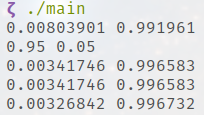
\includegraphics{figures/bayesian_network.png}
  \caption{实验三运行结果}
\end{figure}

\section{讨论及结论}
本次实验我们实现了给定贝叶斯网络和 CPT 计算条件概率。
该实验首先利用输入的文件,构建了一个贝叶斯网络。
然后读取问题文件中的概率问题,利用 CPT 表进行计算。
算法利用二进制编码降低了算法复杂性,但同样也提高了代码的编写难度。
通过此次实验我们更加深入地理解了贝叶斯网络。

\end{document}